\documentclass{article}

\usepackage{graphicx}
\usepackage{listings}
\usepackage{color}
\usepackage[dvipsnames]{xcolor}

\renewcommand\lstlistingname{Quelltext} % Change language of section name

\definecolor{ltgray}{rgb}{0.98,0.98,0.98}

\lstset{ % General setup for the package
    backgroundcolor=\color{ltgray},  
    language=C++,
    numberstyle=\tiny,
    frame=tb,
    tabsize=4,
    columns=fixed,
    showstringspaces=false,
    showtabs=false,
    keepspaces,
    captionpos=bf,
    morekeywords={*,cl_int,cl_platform_id},
    commentstyle=\color{blue},
    keywordstyle=\color{magenta}
}

\title{My OPENCL Notes}
\date{2022-12-25}
\author{cgonzalezbrito}

\begin{document}
  \pagenumbering{gobble}
  \maketitle
  \newpage
  \pagenumbering{arabic}
  \section{Introduction}
  TODO
  \section{Host Programming}
  The program on the host is responsible for the initialization, coordination of kernels execution and data transfer to the kernels. The host creates the initial data buffers that are used by the kernel in charge of normalizing and writing the data into FIFO buffer channels.

 \begin{figure}[h!]
    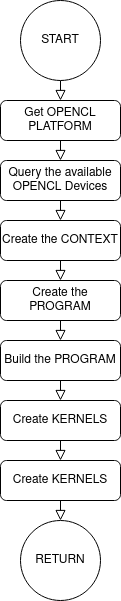
\includegraphics[width=0.2\linewidth]{images/host_diagram.png}
    \caption{Host main diagram}
    \label{fig:Host functions main diagram}
  \end{figure}

  \subsection{Get OpenCL Platform}
  The of Platform is related to the vendor. OpenCL defines a mechanism to identify a specific vendor’s OpenCL implementation in code, i.e. the platform on which the program run. This is important for portability property of OpenCL.

  \begin{lstlisting}
    cl_int clGetPlatformIDs(cl_uint num_entries,
                            cl_platform_id *platforms,
                            cl_uint *num_platforms)
  \end{lstlisting}
  \caption{Normal use}
  \label{lst:Scarpino}

  \

  \begin{lstlisting}
  // Get the OpenCL platform.
  cl_platform_id platform = findPlatform("Altera");
  if(platform == NULL) {
    printf("ERROR:
            Unable to find Altera OpenCL platform.\n");
    return false;
    }
  \end{lstlisting}
  \caption{VPNC use}

\end{document}
